



\section{部屋利用者の入退室時刻の評価実験}\label{3.3}
滞在ウォッチで記録された部屋利用者の入退室時刻が正確に記録されているか,ビーコンが電池切れをせずに記録されているかを確認するための評価実験を行う.
滞在ウォッチのシステム構成でも説明した通り,受信機がビーコンの電波を受信する間隔は3分である.
そのため,滞在ウォッチで記録される入退室時刻は実際に入退室した時刻と比べて誤差が3分以内であるのが望ましい.
また在室管理プラットフォームであるため,来訪した部屋利用者全員の在室者情報が記録されてなければいけない.
電池切れをせずに正確に記録されているか,電池切れをしている利用者がどれくらいいるかを見る.

本研究で使用しているビーコンは,電池で動作しているため,電池切れの際は電池交換をする必要がある.
電池が切れていると在室者情報は記録できないため,ビーコンの電池が切れているかどうかを通知する必要がある.
通知をする手段としてSlackでの通知を行う.
実際に電池切れを通知した際の様子を図\ref{batoff}に示す.
Slackでの通知を行う理由として,研究室に所属する人全員がSlackを通して連絡やコミュニケーションをとっているからである.
電池切れ通知は,5日以上受信機がビーコンの電波を検知できない人にする.
5日以上の理由として,本研究室では火曜日と金曜日にミーティングが行われるため,5日以上間隔が開く場合は電池切れの可能性が高いからである.
しかし図\ref{batoff}のように,100日以上検知できていないにも関わらず,電池交換がされていない利用者がいる.
電池交換をしていない利用者の特徴として,研究室にこないため電池交換をそもそもしない,通知が来ても電池交換が面倒でそのままにするのが挙げられる.
そのため電池切れの通知だけでは電池交換を行ってくれない可能性がある.
また,Slackでの通知のみでは利用者がメッセージの重要度を低く見積もる可能性があるため,管理者からも利用者に対し適宜コンタクトを取る必要があると考える.
電池切れの通知による電池交換の実行率や完了率を増やすには,改善点として通知頻度の見直しが挙げられる.

\begin{figure}[H]
  \begin{center}
    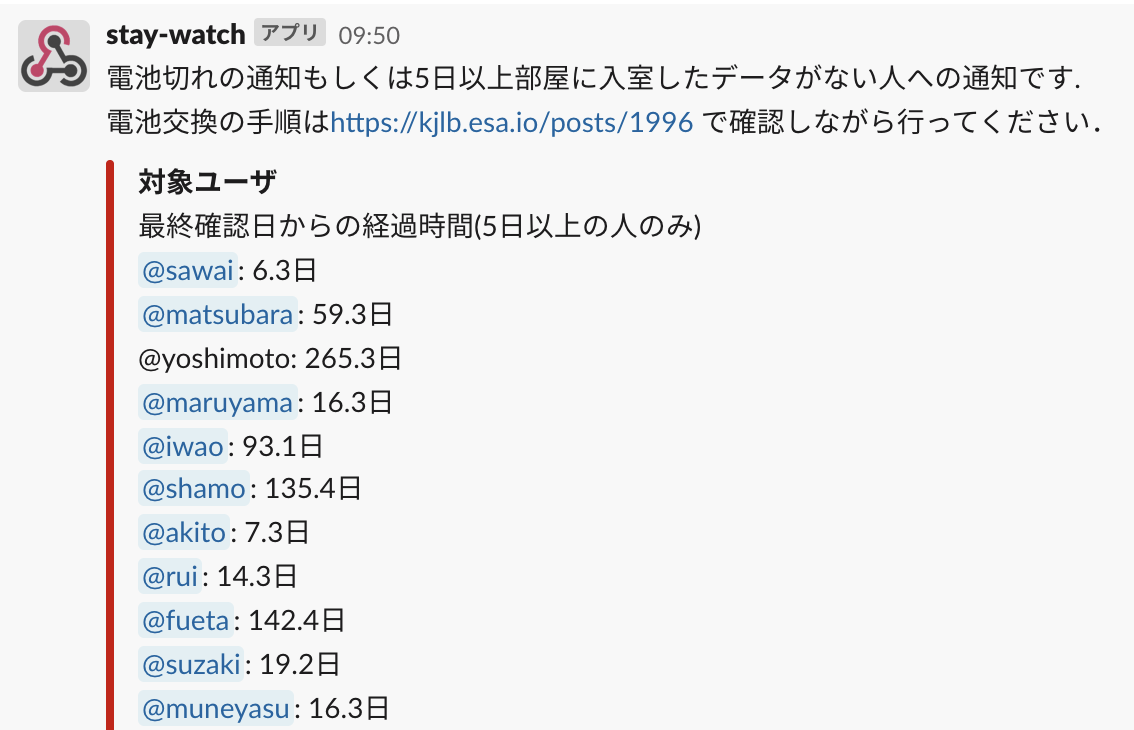
\includegraphics[width=160mm]{image/batoff.png}
    \caption{Slackによる電池切れ通知の実際の様子}
    \label{batoff}
  \end{center}
\end{figure}

2022年1月11日に入退室した13人の部屋利用者と時刻をビデオで撮影し,実際に入退室した時刻と滞在ウォッチで記録された時刻を比較する.
比較した結果を表\ref{actualTimeEstimationTime},表\ref{actualTimeEstimationTime2}に示す.
比較結果として入室時刻の平均誤差が1分.退室時刻の平均誤差が2分であった.
3分毎に受信機がビーコンの電波を検知するので,3分以内の誤差であれば十分な精度であると考える.
しかし,来訪したにも関わらず,記録されていない利用者もいた.
今回在室者情報が記録された利用者は13人,記録できなかった利用者は7人であった.
つまり,記録できなかった利用者は電池切れの通知をしても電池交換をしなかったと考えられる.
今後の課題として,在室者情報が記録できなかった利用者に対してアンケートを行い,なぜ電池交換をしないのか,どのような電池切れ通知するべきか,通知方法,通知頻度を聞く必要がある.
\begin{table}[H]
  \centering
  \caption{実際の入退室時刻と滞在ウォッチで記録された時刻の比較}
  \label{actualTimeEstimationTime}
  \begin{tabular}{|c|c|c|}
    \hline
            & 実際に入退室した時刻   & 滞在ウォッチで記録された     \\
            &                        & 入退室時刻                   \\
    \hline
            & 入室時刻 退室時刻      & 入室時刻\hspace{5mm}退室時刻 \\
    \hline
    利用者A & 09:01\hspace{7mm}10:51 & 09:03:15\hspace{6mm}10:53:13 \\
    利用者B & 08:43\hspace{7mm}10:27 & 08:44:56\hspace{6mm}10:31:50 \\
    利用者C & 08:25\hspace{7mm}10:27 & 08:26:37\hspace{6mm}10:31:50 \\
    利用者D & 10:20\hspace{7mm}19:43 & 10:22:40\hspace{6mm}19:46:05 \\
    利用者E & 10:46\hspace{7mm}14:51 & 10:47:06\hspace{6mm}14:53:59 \\
    利用者F & 10:43\hspace{7mm}13:31 & 10:44:03\hspace{6mm}13:34:54 \\
    利用者G & 10:46\hspace{7mm}15:30 & 10:47:06\hspace{6mm}15:33:30 \\
    利用者H & 10:52\hspace{7mm}12:43 & 10:53:13\hspace{6mm}12:46:12 \\
    利用者I & 10:25\hspace{7mm}14:40 & 10:25:43\hspace{6mm}14:41:48 \\
    利用者J & 10:05\hspace{7mm}15:26 & 10:07:24\hspace{6mm}15:30:28 \\
    利用者K & 12:05\hspace{7mm}18:25 & 12:06:30\hspace{6mm}18:26:58 \\
    利用者L & 10:28\hspace{7mm}14:29 & 10:28:46\hspace{6mm}14:32:41 \\
    利用者M & 12:05\hspace{7mm}17:26 & 12:06:30\hspace{6mm}17:29:11 \\
    \hline
  \end{tabular}
\end{table}
\begin{table}[H]
  \centering
  \caption{実際の入退室時刻と「滞在ウォッチ」で記録された時刻の平均絶対誤差}
  \label{actualTimeEstimationTime2}
  \begin{tabular}{|c|c|}
    \hline
    入室した時刻の平均絶対誤差 & 退室した時刻の平均絶対誤差 \\
    \hline
    1分                        & 2分                        \\
    \hline
  \end{tabular}
\end{table}